
% this file is called up by thesis.tex
% content in this file will be fed into the main document

%: ----------------------- introduction file header -----------------------
%\usepackage{romannum}
\chapter{Introduction} \label{ch1}

% the code below specifies where the figures are stored
\ifpdf
    \graphicspath{{1_introduction/figures/PNG/}{1_introduction/figures/PDF/}{1_introduction/figures/}}
\else
    \graphicspath{{1_introduction/figures/EPS/}{1_introduction/figures/}}
\fi

% ----------------------------------------------------------------------
%: ----------------------- introduction content -----------------------
% ----------------------------------------------------------------------



%: ----------------------- HELP: latex document organisation
% the commands below help you to subdivide and organise your thesis
%    \chapter{}       = level 1, top level
%    \section{}       = level 2
%    \subsection{}    = level 3
%    \subsubsection{} = level 4
% note that everything after the percentage sign is hidden from output



\theoremstyle{definition}
\newtheorem{definition}{Definition}[section]

\section{Introduction} \label{intro} % section headings are printed smaller than chapter names
% intro
Businesses and corporations are in need to develop their relationships with customers, and this happens by improving their business processes that need to be analyzed and assessed to get a significant improvement. Advanced technologies such as process mining and predictive process monitoring can play an essential role in evaluating, and analyzing business processes.

\subsection{Process mining}
A \textit{business process} is defined as a combination of interrelated events, actions, and decisions that point at satisfying certain predefined results or enterprise objectives \cite{dumas2008business}. A \textit{business process} model is a conceptual design of a specific business process \cite{weske2007business} and describes what input we received from the world and how software systems should react  \cite{van2016data}. \textit{Process mining} goes beyond traditional dashboard for performance monitoring, and it is not focusing only on performance measures, e.g. numerical aggregates of performance, but it goes inside the box and opens it to dive into processes, activities, flows, and decisions to explain why the performance we are observing is the one that we are observing, and it connects the gap among regular process model outline and data-driven analysis, e.g. data mining, ML, and business intelligence (BI). At the core of any process mining technique (see figure \ref{fig:pm1}), we have an \textit{event log}, i.e. data we extracted from enterprise systems that contain information or transactions related to a given business process. e.g. \textit{loan application},  and from there, we can do four types of operations. (\romannumeral 1) we can discover a business process model from the event log \textit{(discovery)}; (\romannumeral 2) If we have an event log and a process model we can compare them effectively and verify if the process model conforms to the event log or vice versa, e.g. the observed reality coincides with going to capture the process model \textit{(conformance)}; (\romannumeral 3) Imagine if we have two event logs, e.g. the first one contains all cases when a customer was happy, and the second one contains all cases where a customer complained, and we need to understand what is the difference between the two logs \textit{(variant analysis)}; (\romannumeral 4) Sometimes we have an existing process model with an event log, and we endeavour to describe the performance of the process on top of the process model \textit{(performance mining)}. Interaction between world related systems, e.g. people, machines, and business processes that interact with software-related systems, e.g. bank and transportation systems leads to generate a huge amount of data that we call \textit{event logs} that need to be analyzed and assessed.


%\begin{figure}[htb]
%	\begin{center}
%		\resizebox{\textwidth}{!}{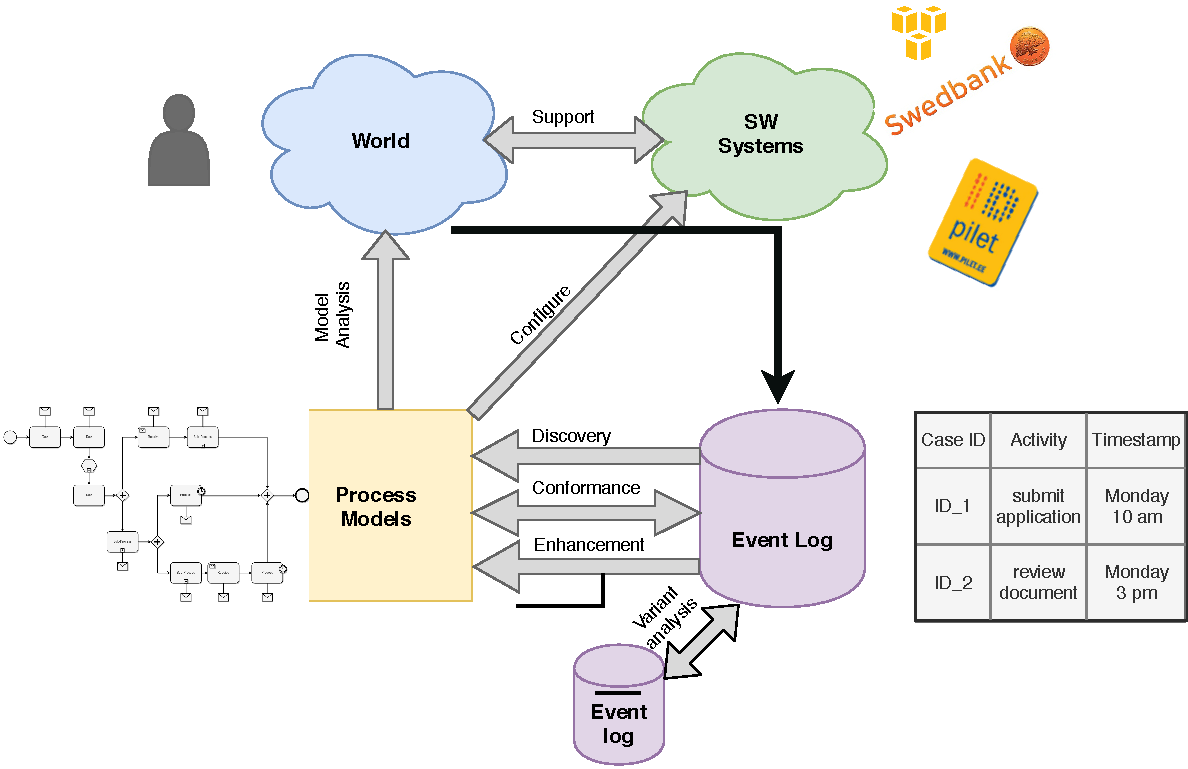
\includegraphics{images/general/pm1.pdf}}
%		\caption{Process mining life cycle}
%		\label{fig:pm1}
%	\end{center}
%\end{figure}

\begin{figure}[htb]
	\begin{center}
		\resizebox{\textwidth}{!}{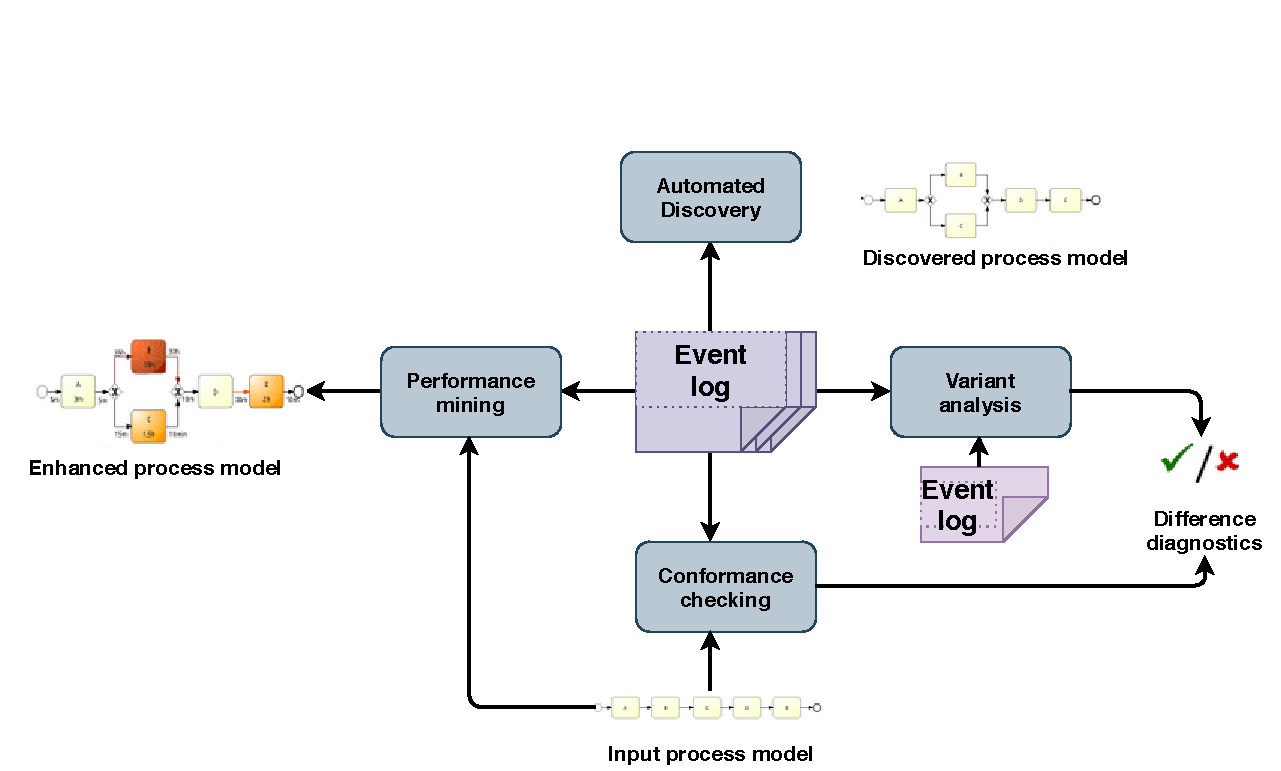
\includegraphics{images/general/pm_new.pdf}}
		\caption{Process mining four main components \cite{dumas2013fundamentals}}
		\label{fig:pm1}
	\end{center}
\end{figure}


An \textit{event log}  (see figure \ref{fig:el} ) is data we extracted from enterprise systems that contain information or transactions related to a given business process. e.g. \textit{loan application} and it’s considered as a set of \textit{cases (or traces)}, e.g. starting by submitting an application, making an offer until reach to an end state with acceptance or cancellation of the application. Each trace consists of a sequence of \textit{events ( or activities}), e.g. submit application, review document, etc., where each event in the trace belongs to the same case. Every event in the trace carries information about an \textit{activity name} (describes what happened?), \textit{timestamp} (indicates when an activity happened?), \textit{resource} (who did the work?), and \textit{life cycle} of an event (start and end of the activity). Event log attributes can be classified into two general groups (see figure \ref{fig:attr}) \cite{teinemaa2019outcome}. (\romannumeral 1) \textit{Control flow}, and it contains the core attributes for any event log, e.g. \textit{case id} (i.e. a unique identifier for a business process), \textit{activity} (i.e. any action that can be done during the execution of business process), \textit{timestamp} (i.e. start and end time for an activity); (\romannumeral 2) \textit{Data payload} that refers to all other attributes of an event log, e.g. \textit{name, age, etc.} 

\begin{figure}[1htbp]
	\begin{center}
		\resizebox{9cm}{!}{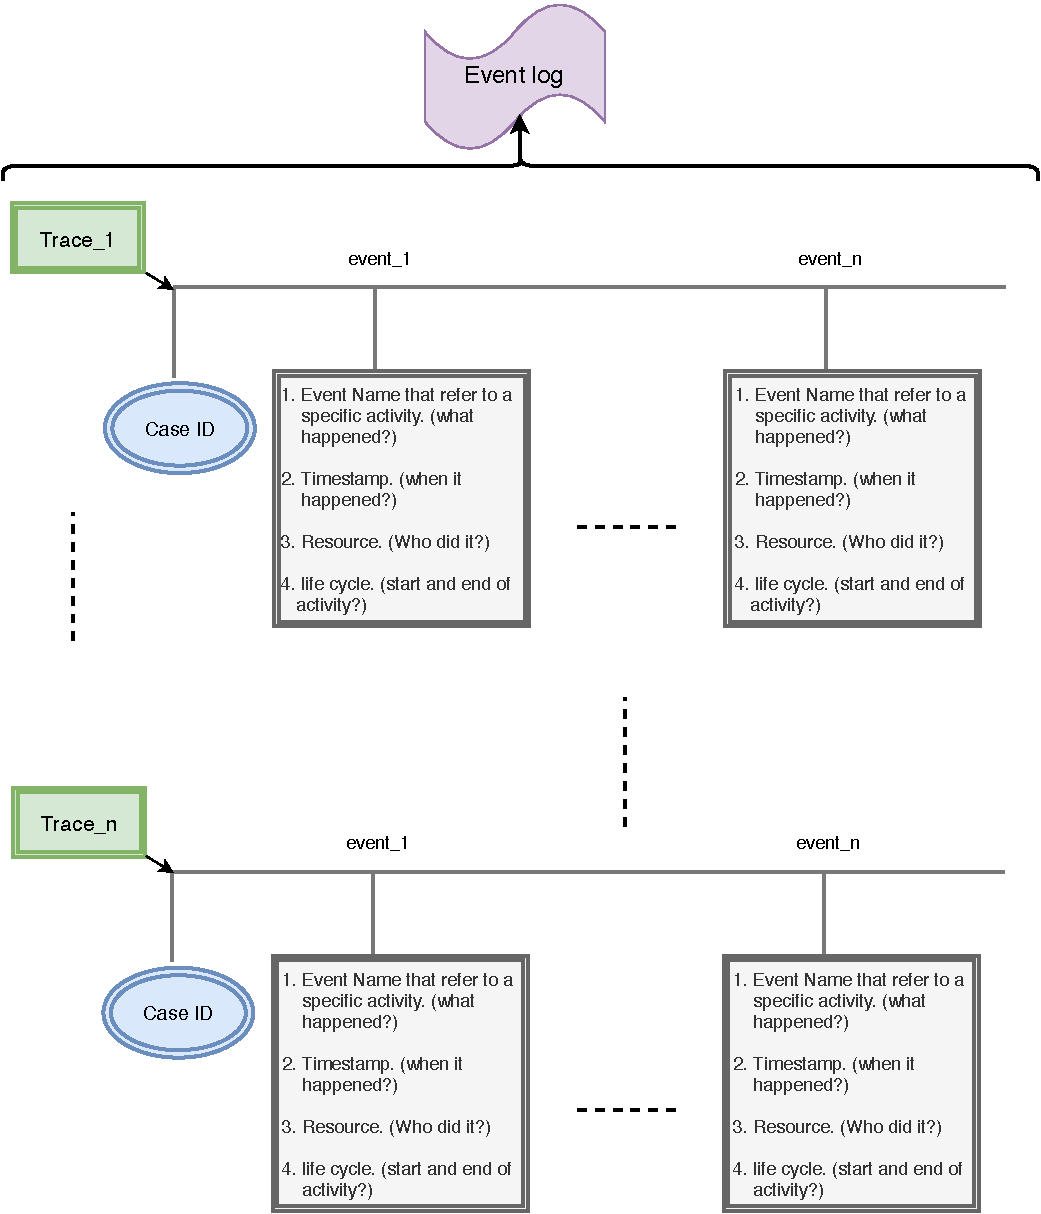
\includegraphics{images/general/et.pdf}}
		\caption[Event log]{Event log: consists of a set of traces, and each trace contains information about its control flow and data payload.}
		\label{fig:el}
	\end{center}
\end{figure}


\begin{figure}[htb]
	\begin{center}
		\resizebox{10cm}{!}{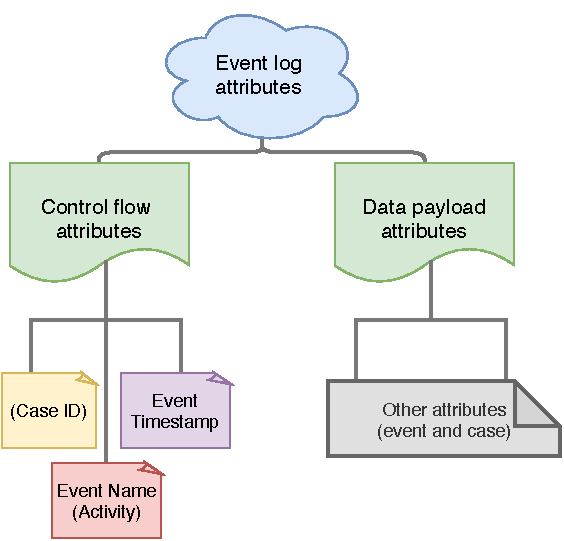
\includegraphics{images/general/attr.pdf}}
		\caption{Event log attributes}
		\label{fig:attr}
	\end{center}
\end{figure}



\theoremstyle{definition}
\begin{definition}{\textit{\textbf{Event}}}
	Assume $E$ holds the universe of all possible events, and $ \forall e \in E: e = \{a, c, t, (m_1, ..., m_n)\}$ as $a$ refers to an activity name; $c$ is a unique identifier of a business case (or case id); $t$ refers to the timestamp; finally, $m$ represents all other attributes where $n > 0$
\end{definition}


\begin{definition}{\textit{\textbf{Trace}}}
	Let $R$ be the universe of all traces and $\forall \sigma \in R,  \sigma$ is a sequence of events such that $\sigma = (e_1, ..., e_n)$, where all events in $ \sigma $ belong to the same case (see figure \ref{fig:el}).
\end{definition}

\begin{definition}{\textit{\textbf{Event log}}}
	An event log $L$ is a collection of complete business cases (or traces) $L=\{\sigma_1, ..., \sigma_n \}$
	
\end{definition}

Enterprises use process mining procedures with an event log as an input to answer a variety of key questions such as What is the process that people follow? And Where the bottlenecks in business processes? And Why? Where people deviate from the expected or idealized process? And Why? However, the process mining techniques presented above are focused on analyzing historical data and extracting insights about the general behaviour of the process. These techniques do not help us to monitor ongoing process instances nor to determine what will happen next? This latter question is addressed by a complementary set of process mining techniques known as \emph{predictive process monitoring}.

% Can we detect problems, e.g. delay, deviation, risk, etc. for ongoing business cases. 

\subsection{Predictive process monitoring(PPM)}
\textit{Predictive process monitoring} (PPM) is a part of process mining and designed to help organizations and enterprises on a daily level. PPM takes a historical event log as an input (see figure \ref{fig:pmwf}) to build predictive models in the \textit{offline} step then in the \textit{online} phase we produce a stream of predictions based on a given stream of events about different ongoing business cases. In PPM given an \textit{incomplete trace} (or running case) (see figure \ref{fig:runtr}) different measures of interest can be predicted \cite{senderovich2019knowledge}, e.g. outcome,  next activity, or the remaining time for ongoing or running cases at their execution time. In this thesis, we are focusing on \textit{outcome-oriented} PPM, which means we aim to predict the outcome for an incomplete trace. In this context, we define a prefix function as $P(\sigma, k)$ to return the prefix of a trace with size $k$.


\begin{figure}[htb]
	\begin{center}
		\resizebox{10cm}{!}{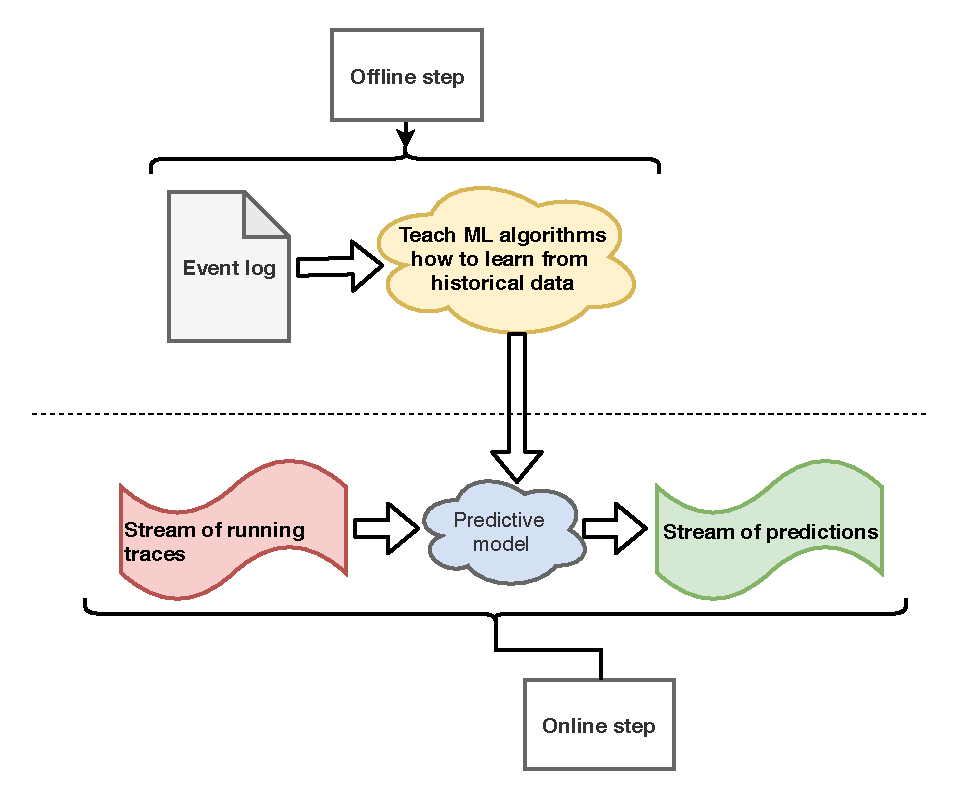
\includegraphics{images/general/pmwf.pdf}}
		\caption[Predictive process monitoring workflow]{A general overview of predictive process monitoring workflow with its two main steps, i.e. offline (or training), and online (or prediction).}
		\label{fig:pmwf}
	\end{center}
\end{figure}

\begin{figure}[htb]
	\begin{center}
		\resizebox{10cm}{!}{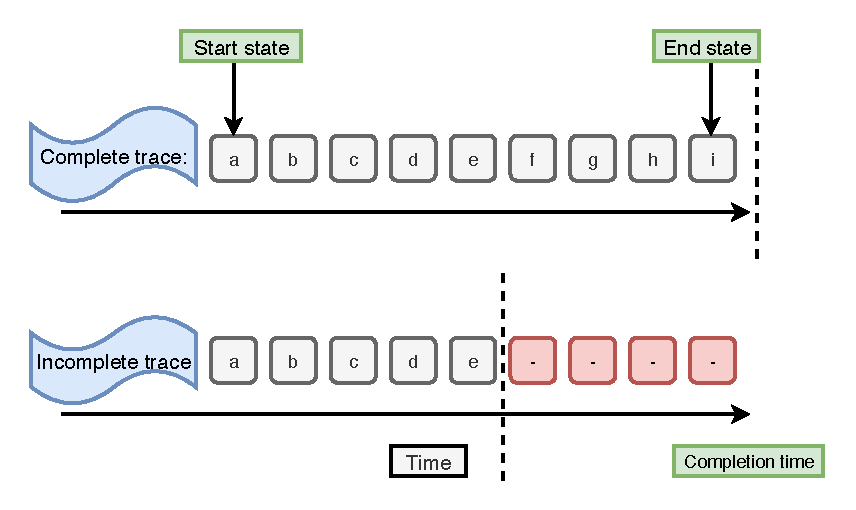
\includegraphics{images/general/runtr.pdf}}
		\caption[Complete and incomplete trace]{Difference between complete (i.e. it reaches to an end state) and incomplete (or running ) trace \cite{teinemaa2019outcome}.}
		\label{fig:runtr}
	\end{center}
\end{figure}

\begin{definition}{\textit{\textbf{Prefix function $P$}}}
	Given a complete trace $\sigma = (e_1, .., e_n)$ where $k < n$, and $k \in \mathbb Z^+$, then $P(\sigma, k) = (e_1, ..., e_k)$
	
\end{definition}


Organizations and enterprises have many different business goals \textit{(outcomes)} based on their objectives, e.g. is a customer complaint or not. Accordingly, the outcome of a trace is determined using several methods based on business targets. An outcome can be \textit{categorical} (i.e. discrete values, e.g. will the customer accept or decline a bank offer) or \textit{numerical} (i.e. continuous values, e.g. invoice amount). In a business environment, it’s more suitable to define outcome classes as a binary variable with only two possible states that give information about if the ongoing case will end with an expected (i.e. $ve^{+}$, e.g. customer accepts the bank offer) or unexpected (i.e. $ve^{-}$, e.g. customer declines the offer)  outcome.  In this thesis, we deal with a categorical binary outcome for any business process monitoring task. To determine the outcome for a business case, we define a \textit{target function $f$}.

\begin{definition}{\textit{\textbf{Target function $f$}}}
	A target function $f: R \to y$ maps all complete traces to its target class such that $\forall \sigma \in R$, then $f(\sigma) \in y$ where $y=\{1,0\}$
	
\end{definition}

Outcome-oriented PPM problems are usually solved by teaching ( or training ) a machine learning (ML) algorithm on how to learn from historical data, e.g. event log (see figure \ref{fig:pmwf}). A \textit{predictive model} will result after the training phase, and then this model will be evaluated using test data (i.e. portion form historical event log). If the resulting model acts accurately on unseen (or test) data with acceptable accuracy, then it will be deployed to monitor the running cases in real-life which guides us to investigate how to improve existing PPM techniques in terms of performance. 


\newcommand{\quotes}[1]{``#1''}


\subsection{Problem statement}
This work answers the question of \quotes{How to improve the existing outcome-oriented predictive process monitoring methods?}.
The mentioned research question has been examined for a long time, which enriches the area of outcome-oriented predictive monitoring.  Existing methods of predictive process monitoring have the same objective to improve business process performance. In this thesis, (\romannumeral 1) we revisit most of the existing approaches for PPM \cite{teinemaa2019outcome}; (\romannumeral 2) Introduce three methods to improve the outcome-oriented PPM; (\romannumeral 3) Create a benchmark of $20$ different PPM tasks with the help of real-life event logs; (\romannumeral 4) Build a comparative experimental assessment of the existing and proposed methods utilizing this benchmark. 

 In this thesis, we combine and introduce three new approaches to improve the existing outcome-oriented PMM techniques.


\subsection{Contributions}

This work proposes three contributions to the area of outcome-oriented predictive process monitoring. 

\noindent \textbf{Contribution $1$:}  Introducing a machine learning algorithm (i.e. \textit{CatBoost}) \cite{prokhorenkova2018catboost} that handles categorical attributes automatically to outcome-oriented predictive process monitoring methods. \textit{CatBoost} is a recently gradient boosting method and an open-source machine learning algorithm where its name has two main words that describe its features \quotes{\textbf{Cat}egory}, and \quotes{\textbf{Boost}ing}. \\

\noindent \textbf{Contribution $2$:} Proposing a complex sequence encoding method based on \textit{discrete wavelet transformation} \cite{edwards1991discrete} and time-series encoding. In this encoding process, we encode each trace in the event log into a collection of vectors with an equal length for each event in our log. In this contribution we used \textit{neural networks auto-encoders} to reduce the dimensionality of the generated feature vector then we added this vector to other simple sequence encoding methods as a way to improve the overall performance of predictive monitoring in terms of accuracy.  \\

\noindent \textbf{Contribution $3$:} In real-life systems, the final outcome of an ongoing business process relies on the interaction between all business cases that are working concurrently at the same time \cite{senderovich2019knowledge}. In this context, we propose new \textit{inter-case} features that capture information about: (\romannumeral 1) \emph{Workload}, e.g. a number of cases that have started and did not finish; (\romannumeral 2) \emph{Demand intensity}, e.g. how many cases were created since the current case started divided by a number of seconds since the running case was created; (\romannumeral 3) \emph{Temporal context}, e.g. day of the week when the last event in the current case occurred.


This thesis is constructed as follows. In Chapter \ref{ch2}: we present the significant concepts and standards of machine learning to build a predictive model.  Chapter \ref{ch3}: we summarize the literature for current outcome-oriented PPM methods.  In Chapter \ref{ch4}: we propose our approaches to improve predictive process monitoring techniques. Chapter \ref{ch5} we build the benchmark and conduct a comparative empirical evaluation. Lastly, Chapter \ref{ch6} summarizes this thesis with a review of our proposed methods and addressing possible later improvement.














